\documentclass[conference]{IEEEtran}
\ifCLASSINFOpdf
\else
\fi
\hyphenation{op-tical net-works semi-conduc-tor}
\usepackage{graphicx}


\begin{document}

\title{Data Analysis Project-NBA Winner Prediction}

\author{\IEEEauthorblockN{Semih İpek}
\IEEEauthorblockA{Computer Engineering 3rd year\\
University of Galatasaray\\
Istanbul, Turkey\\
semih.ipek@ogr.gsu.edu.tr\\
}}

\maketitle
\IEEEpeerreviewmaketitle

\section{Introduction}

\subsection{Overview}
The National Basketball Association is the largest basketball association in the world and brings in an estimated eight billion dollars a year. As a collective whole, the NBA generates immense revenue and data. The data pertains to teams and players alike. This data is beneficial for analytics and game strategy. Sports teams and organizations have adapted data analytics and modeling to gain every competitive advantage they can get. A lot of decisions made in a basketball game are determined by statistics and analytics. These analytics could very well make the difference in the outcome of a game. 
Sport predictions have been becoming more relevant in the industry. Before every game, analysts will display a prediction as to who will win and the margin of victory. Another industry that has stemmed from sport predictions is the betting industry. Legal betting platforms have been appearing and expanding for years. An accurate model is imperative to predict games and quantify all metrics in a basketball game to ensure the betting process is equitable. There are many uses to machine learning models in sports and their usefulness is only growing.


\subsection{Motivation}

The purpose of this analysis is to harness the power of data to enhance the understanding of factors influencing game outcomes. Through comprehensive data analysis encompassing team statistics, player performances, historical trends, and game dynamics, the aim is to create predictive models that can forecast potential winners more accurately. By delving into the wealth of data available in the NBA, this analysis seeks to uncover patterns and correlations that contribute significantly to determining match results.
\subsection{Research Questions}


\subsubsection{Main Question}


\vspace{\baselineskip}
\paragraph {Who will win?}
Determining the winner of a match involves considering countless variables. It's a complex interplay of factors that makes predicting outcomes a lucrative pursuit. To assess the potential winner, let's delve into some of the influential elements affecting the match's outcome.






\vspace{\baselineskip}

\subsubsection{Sub-questions}
\vspace{\baselineskip}
\vspace{\baselineskip}
\vspace{\baselineskip}

\paragraph {Which team is better?}

This question carries weight because, as we've pointed out, each match has its own twists and turns. That's the main reason we see score differences .

\paragraph {Which teams exhibit the highest field goal percentage (FG\%), three-point percentage (3P\%), and free throw percentage (FT\%)? How do these percentages correlate with their overall points scored per game? }

\vspace{\baselineskip}
\paragraph {How do teams compare in terms of two-point field goal percentage (2P\%) versus three-point field goal percentage (3P\%)? Are there teams that heavily rely on one type of scoring over the other?
}
\vspace{\baselineskip}
\paragraph {Which teams exhibit strong passing and ball control, as seen in their assist (AST) to turnover (TOV) ratio? How does this ratio impact their offensive efficiency? }
\vspace{\baselineskip}

\paragraph {Which teams perform well in defensive statistics such as steals (STL) and blocks (BLK)? Is there a correlation between them? }

\vspace{\baselineskip}
\paragraph {Which teams get more rebounds? Does it have a relation with FG\%? }
\vspace{\baselineskip}

\section{Method}
\subsection{Dataset}
\subsubsection{Story/Overview}
Contained within this dataset lies a comprehensive compilation of statistical records from the 2022-2023 NBA Season, spanning 30 teams and capturing the essence of their performance across an entire season. With 82 observations for each team, this dataset encompasses a treasure trove of basketball metrics, ranging from shooting accuracy to defensive strategies, offering an extensive view of team dynamics and gameplay strategies. With a focus on fundamental aspects like field goal percentages, three-point shooting prowess, free throw efficiencies, rebounds, assists, steals, and turnovers, this dataset serves as a goldmine for unraveling the multifaceted facets that define the competitive landscape within the NBA. 
\vspace{\baselineskip}
\vspace{\baselineskip}
\vspace{\baselineskip}

\subsubsection{Attributes}
\begin{flushleft}
\begin{tabular}{@{}ll@{}}
  
    Rk: &The rank of the team\\
    Team: &The name of the team.\\
    G: &Number of games played.\\
    MP: &Minutes played.\\
    FG: &Field goals made.\\
    FGA: &Field goals attempted.\\
    FG\%: &Field goal percentage.\\
    3PM: &Three-pointers made per game on average.\\
    3PA: &Three-point attempts per game on average.\\
    3P\%: &Three-point percentage.\\
    2P: &Two-pointers made per game on average.\\
    2PA: &Two-point attempts per game on average.\\
    2P\%: &Two-point percentage\\
    FT: &Free throws made per game on average.\\
    FTA: &Free throw attempts per game on average.\\
    FT\%: &Free throw percentage.\\
    ORB: &Offensive rebounds per game on average.\\
    DRB: &Defensive rebounds per game on average.\\
    TRB: &Total rebounds per game on average.\\
    AST: &Assists per game on average.\\
    STL: &Steals per game on average.\\
    BLK: &Blocks per game on average.\\
    TOV: &Turnovers per game on average.\\
    PF: &Personal fouls committed per game on average.\\
    PTS: &Points scored per game on average.\\
\end{tabular}
\end{flushleft}

\section{Result}
\subsection{Descriptive Analysis }
We have all the 30 team from NBA (National Basketball Association) and their data about different stats.So let’s take a look at data  that we have and examine some of the analysis.
There are 25 columns but we will only use 11 of them which are necessary for our analysis.
\vspace{\baselineskip}
\vspace{\baselineskip}

\vspace{\baselineskip}
\vspace{\baselineskip}
\begin{tabular}{|l||c|r|}
    \hline
    \multicolumn{3}{|c|}{Overview of DataFrame} \\
    \hline
    Column & Non-Null Count & Type \\
    \hline
    Rk & 30 & Ordinal \\
    Team & 30 & Nominal \\
    G & 30 & Numerical \\
    MP & 30 & Numerical \\
    FG & 30 & Numerical \\
    FGA & 30 & Numerical \\
    FG\% & 30 & Numerical \\
    3PM & 30 & Numerical \\
    3PA & 30 & Numerical \\
    3P\% & 30 & Numerical \\
    2P & 30 & Numerical \\
    2PA & 30 & Numerical \\
    2P\% & 30 & Numerical \\
    FT & 30 & Numerical \\
    FTA & 30 & Numerical \\
    FT\% & 30 & Numerical \\
    ORB & 30 & Numerical \\
    DRB & 30 & Numerical \\
    TRB & 30 & Numerical \\
    AST & 30 & Numerical \\
    STL & 30 & Numerical \\
    BLK & 30 & Numerical \\
    TOV & 30 & Numerical \\
    PF & 30 & Numerical \\
    PTS & 30 & Numerical \\
    \hline
\end{tabular}

\vspace{\baselineskip}

\vspace{\baselineskip}

\begin{tabular}{|l||c|r|}
    \hline
    \multicolumn{3}{|c|}{Overview of DataFrame} \\
    \hline
    Column & Non-Null Count & Type \\
    \hline

    FG\% & 30 & Numerical \\
    3PM & 30 & Numerical \\
    3P\% & 30 & Numerical \\
    2P\% & 30 & Numerical \\
    FT\% & 30 & Numerical \\
    TRB & 30 & Numerical \\
    AST & 30 & Numerical \\
    STL & 30 & Numerical \\
    BLK & 30 & Numerical \\
    TOV & 30 & Numerical \\
    PTS & 30 & Numerical \\
    \hline
\end{tabular}

\vspace{\baselineskip}
\vspace{\baselineskip}
Now, let's analyse the data by using some diagrams which can help us answering our questions.

\vspace{\baselineskip}
\vspace{\baselineskip}
\vspace{\baselineskip}
\vspace{\baselineskip}
\vspace{\baselineskip}


\subsubsection{PTS}

We have data on the average points scored per game by teams throughout the season. Analyzing this information is crucial for predicting team performance. Looking at the distribution, the points scored per game showcase a normal distribution. With a mode of 114.93, a median of 114.30, and a mean of 114.69, these values indicate a relatively close alignment, suggesting a balanced spread of points across teams. It can be stated that there is a normal distribution.
\begin{figure}[h]
    \centering
    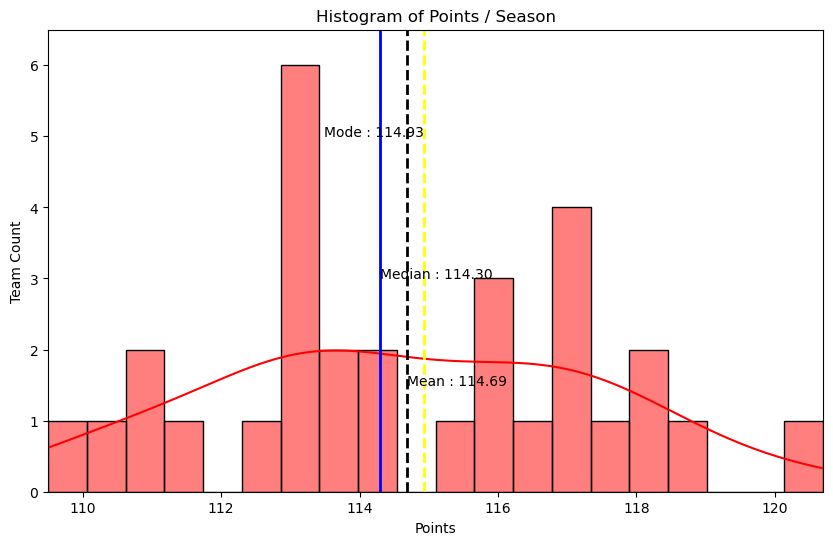
\includegraphics[scale=0.41]{PTS_image.png}
    \caption{Points Per Game}
    \label{fig:enter-label}
\end{figure}

\vspace{\baselineskip}
\vspace{\baselineskip}
\vspace{\baselineskip}
\subsubsection{2P\%}
The histogram illustrates the distribution of 2-Point Field Goal Percentage (2pt\%) across multiple teams, providing an overview of their shooting accuracy. The distribution appears relatively symmetric, centered around an average of 55\%. This suggests that, on average, teams tend to perform consistently in converting two-point shots.The mean 2pt\% across all teams is calculated at 55.0\%, indicating a general trend in shooting accuracy. The median, aligning closely with the mean at 55.0\%, indicates that the distribution isn't skewed by extreme values, portraying a balanced performance across the teams.The mode, representing the most frequent 2pt\% value in the distribution, also aligns closely with the mean and median, signifying a symmetrical pattern in the teams' 2pt\% performance. This consistency suggests a commonality in shooting efficiency across the teams within this range. Finally we can say that we have a normal distribution.


\begin{figure}[h]
    \centering
    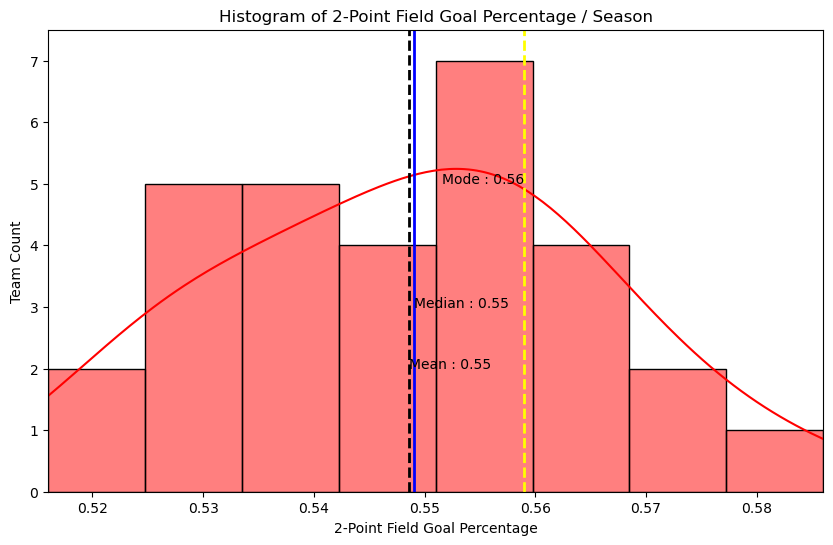
\includegraphics[scale=0.41]{2P_image.png}
    \caption{2-Point Percentage }
    \label{fig:enter-label}
\end{figure}



\vspace{\baselineskip}
\vspace{\baselineskip}
\vspace{\baselineskip}
\vspace{\baselineskip}
\vspace{\baselineskip}
\vspace{\baselineskip}
\vspace{\baselineskip}
\vspace{\baselineskip}
\vspace{\baselineskip}
\vspace{\baselineskip}

\subsubsection{3P\%}
The mode, median, and mean are tightly aligned at approximately 0.36. This coherence suggests that across the teams included in the dataset, there's a consistent performance in terms of 3-point shooting accuracy, clustered around this specific percentage. The histogram's shape indicates a uniform distribution, showcasing that a significant number of teams fall within this relatively narrow range of 3-point shooting accuracy. It's evident that the dataset exhibits a strikingly balanced normal distribution.

\begin{figure}[h]
    \centering
    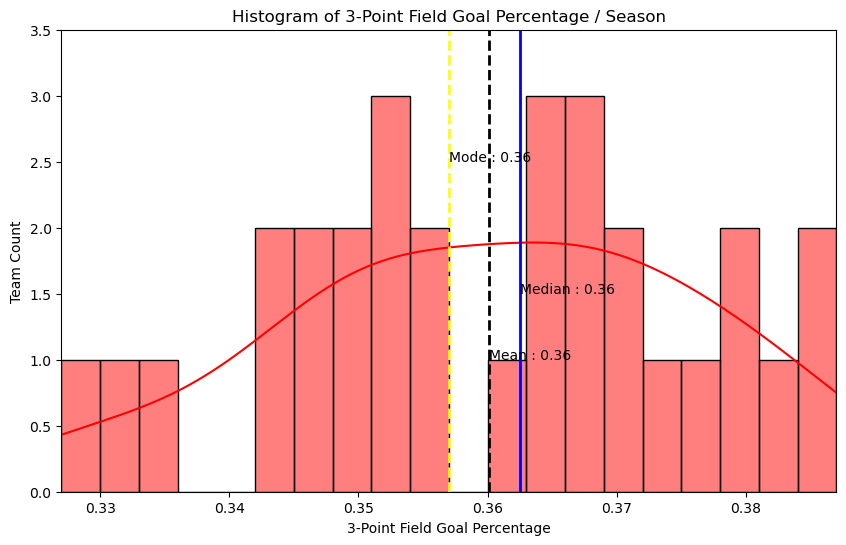
\includegraphics[scale=0.41]{3P_image.png}
    \caption{3-Point Percentage }
    \label{fig:enter-label}
\end{figure}



\subsubsection{3PM}
It reveals an interesting distribution among the teams in the dataset. The mode, median, and mean values(10.80, 12.05, 12.34 respectively) highlight a consistent trend where most teams make around 12 3-pointers per game on average. This alignment suggests a tendency among teams to hit a similar number of 3-pointers, with a majority clustered around this specific range. The histogram indicates that while there's a prevalent cluster around the mean and median values, there are some variations in performance, creating a spread among the teams in terms of 3-point field goals made per season.It seems like we have a distribution skewed to right.

\begin{figure}[h]
    \centering
    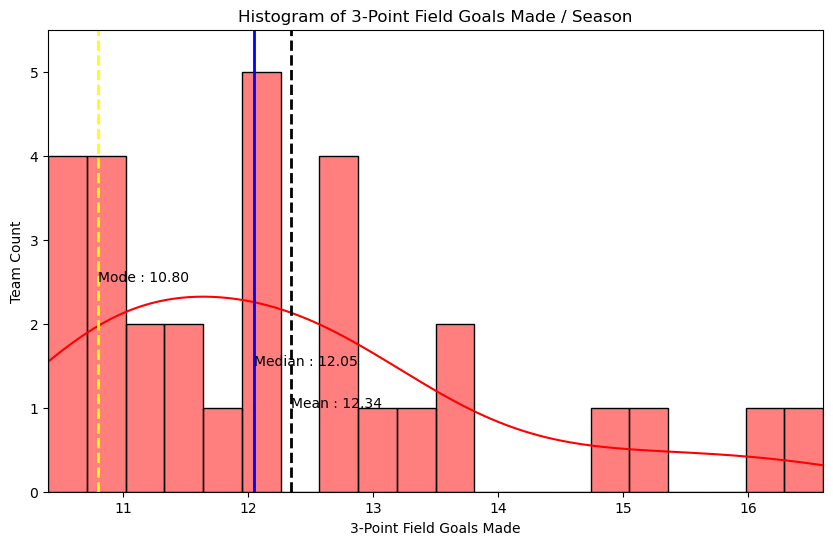
\includegraphics[scale=0.41]{3PM_image.png}
    \caption{3-Points Made Per Game}
    \label{fig:enter-label}
\end{figure}


\subsubsection{AST}
The analysis of Assists (AST) among the teams in the dataset highlights a consistent performance, averaging around 25 assists per season. Assists in basketball signify collaborative play, demonstrating a team's ability to pass and create scoring opportunities for one another. The close alignment of the mode, median, and mean values (25.02, 25.25, and 25.32 respectively) indicates a prevalent trend in team assist counts, showcasing a collective effort in facilitating scoring opportunities for better team performance. We can say that there is a normal distribution.

\begin{figure}[h]
    \centering
    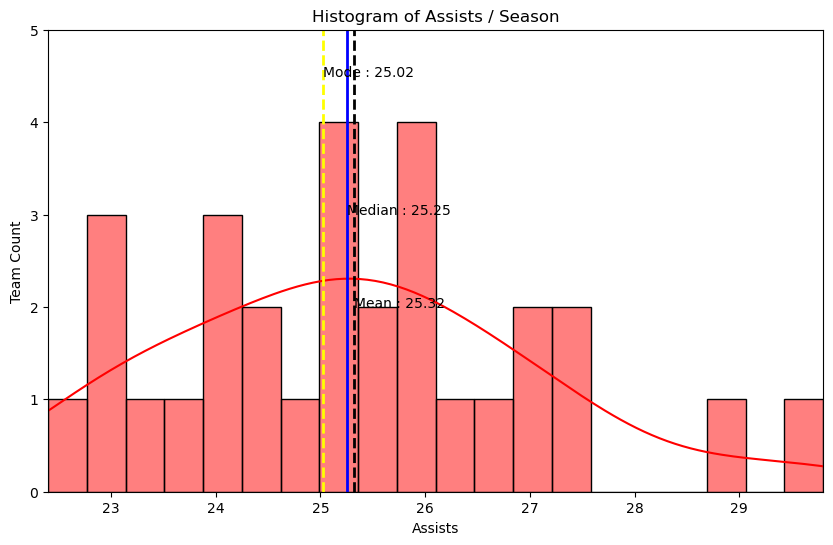
\includegraphics[scale=0.41]{AST_image.png}
    \caption{Assists Per Game }
    \label{fig:enter-label}
\end{figure}
\vspace{\baselineskip}

\subsubsection{BLOCK}
Blocks in basketball are a critical defensive aspect, showcasing a team's ability to deny opponent shots and significantly impact game dynamics. This histogram of Blocks (BLK) reflects defensive strengths across the league's teams, revealing varying degrees of shot-blocking prowess. The mode (5.20), median (4.65), and mean (4.66) values showcase a central tendency in shot-blocking performance across the teams. While these figures provide a general overview, the distribution's shape can also reveal insights. The mode, being close to the mean and median, suggests a relatively balanced distribution of shot-blocking abilities among teams so that the reason why it has a normal distribution. 
\begin{figure}[h]
    \centering
    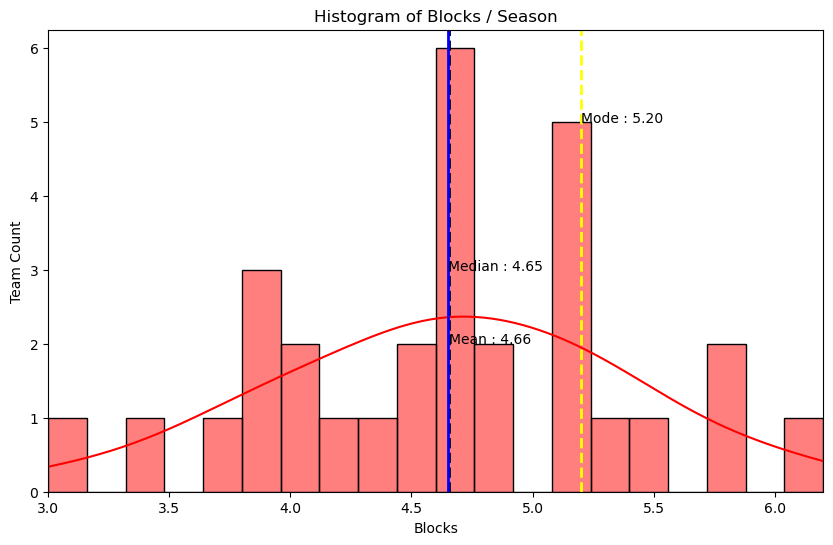
\includegraphics[scale=0.41]{BLOCK_image.png}
    \caption{Blocks Per Game}
    \label{fig:enter-label}
\end{figure}
\vspace{\baselineskip}
\vspace{\baselineskip}


\subsubsection{FG\%}
Field Goal Percentage (FG\%) stands as a critical metric in basketball, reflecting a team's efficiency in converting field goal attempts into successful scores. The histogram portrays a distribution of shooting accuracy among basketball teams. The close alignment between the mode, median, and mean FG\% values at approximately 0.47 to 0.48 indicates a consistent shooting performance across these teams. This consistency in values indicates a competitive landscape where most teams maintain similar shooting efficiency.So it can be stated that there is a normal distribution
\begin{figure}[h]
    \centering
    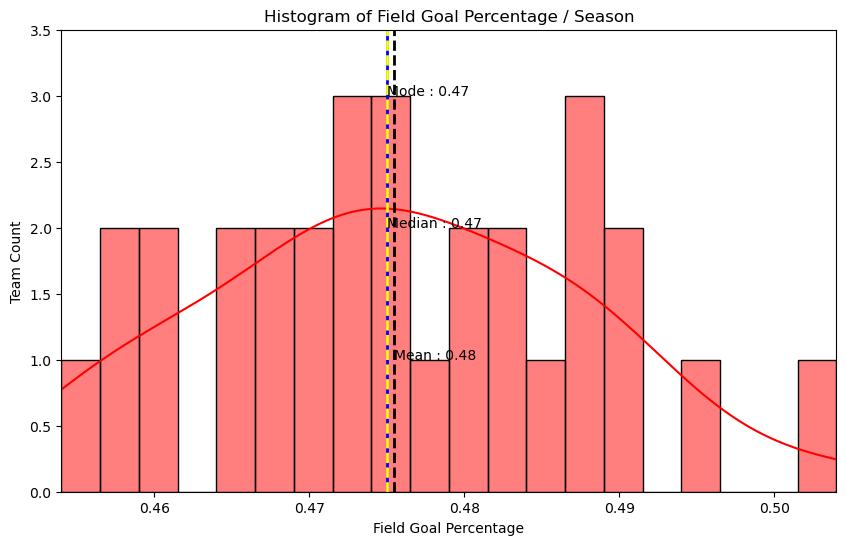
\includegraphics[scale=0.41]{FG_image.png}
    \caption{Field Goal Percentage}
    \label{fig:enter-label}
\end{figure}
\vspace{\baselineskip}
\vspace{\baselineskip}
\vspace{\baselineskip}


\subsubsection{FT\%}
Free Throw Percentage (FT\%) is a vital indicator of a team's accuracy and consistency in converting free throw attempts into points. The histogram showcases the distribution of free throw shooting efficiencies among the teams. The convergence of mode, median, and mean FT\% values around 0.78 suggests a uniform performance level across the dataset and also it has a normal distribution.
\begin{figure}[h]
    \centering
    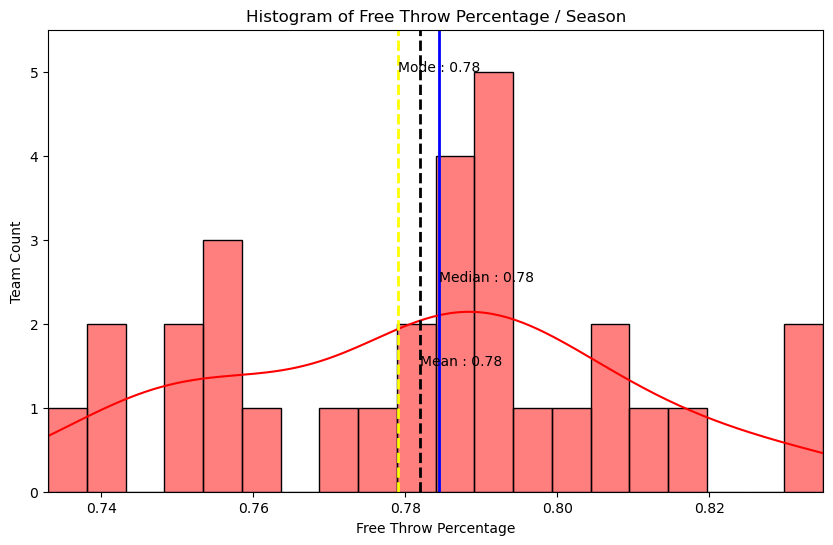
\includegraphics[scale=0.41]{FT_image.png}
    \caption{Free Throw Percentage}
    \label{fig:enter-label}
\end{figure}

\subsubsection{STEAL}
Steals (STL) in basketball signify a team's ability to intercept or disrupt the opponent's plays, crucial for regaining possession. This histogram visualizes the distribution of steals per season among different teams. The mode, median, and mean, hovering around 7.10 to 7.29, showcase a relatively consistent performance level across the dataset. Such uniformity underscores the importance of defensive strategy and quick play disruption in basketball. Teams with higher steal averages often exhibit stronger defensive capabilities, impacting their overall game strategy and potential success. We can say that we have a distribution skewed to right.
\begin{figure}[h]
    \centering
    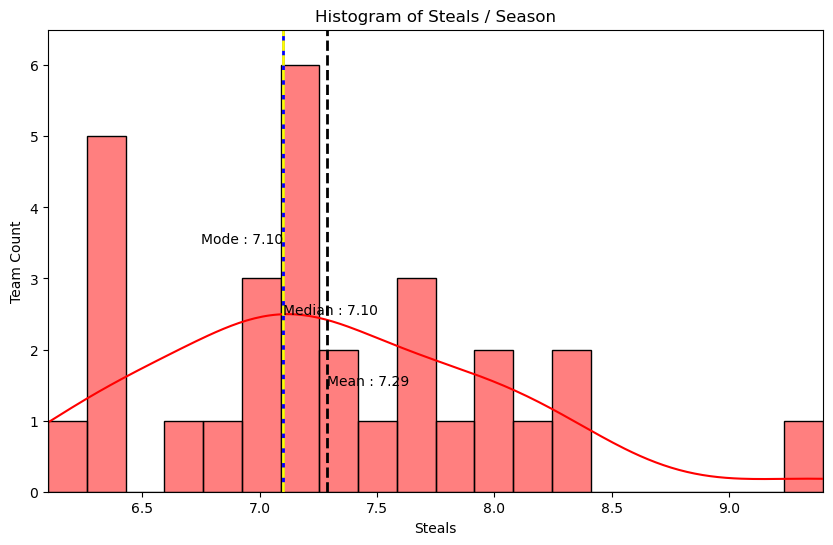
\includegraphics[scale=0.41]{STEAL_image.png}
    \caption{Steals Per Game}
    \label{fig:enter-label}
\end{figure}

\subsubsection{TOV}
Turnovers in basketball signify the loss of possession due to various factors like errors in passing, ball handling, or defensive steals by the opponent. High turnover rates can disrupt a team's offensive rhythm, affecting their scoring opportunities and allowing opponents more possessions. The mode, at 13.50 turnovers, indicates the most frequently occurring value, while both the median and mean are relatively close, standing at 14.10 and 14.09, respectively. This distribution implies that while the most common turnover count is around 13.50, there are instances where turnover rates climb to about 14.10 on average.  The histogram representing turnovers per season displays a  right-skewed distribution.
\begin{figure}[h]
    \centering
    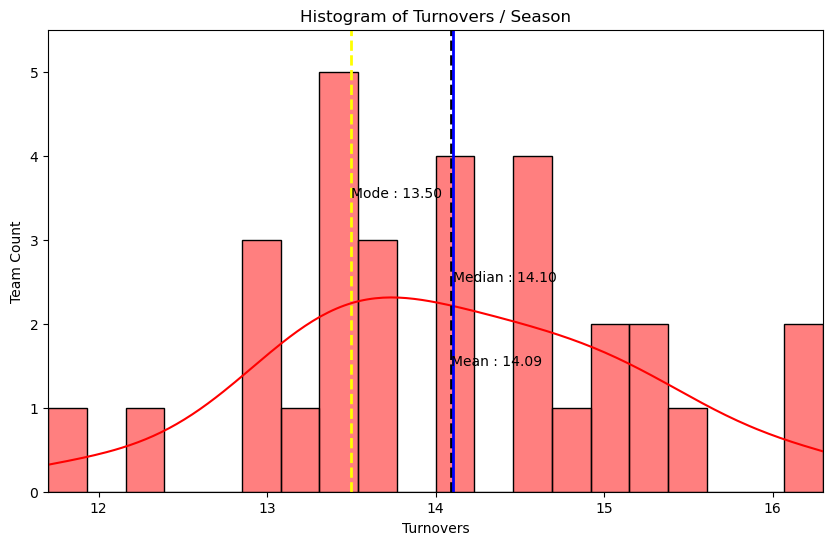
\includegraphics[scale=0.41]{TOV_image.png}
    \caption{Turnovers Per Game}
    \label{fig:enter-label}
\end{figure}

\subsubsection{TRB}
Total rebounds (TRB) are a critical metric in basketball, reflecting a team's ability to retrieve missed shots on both offensive and defensive ends. Total rebounds (TRB) indicate the combined number of rebounds secured by a team over a season. Analyzing the TRB average aids in understanding a team's performance in controlling both offensive and defensive rebounds. In the presented graphic, the mode, median, and mean values(43.29, 43.40, 43.43 respectively) suggest a relatively close alignment, indicating a balanced distribution around the mean value, showcasing consistent team performance in securing rebounds throughout the season. It can be said that there is a normal distribution.
\vspace{\baselineskip}
\vspace{\baselineskip}
\vspace{\baselineskip}
\vspace{\baselineskip}
\vspace{\baselineskip}
\vspace{\baselineskip}

\begin{figure}[h]
    \centering
    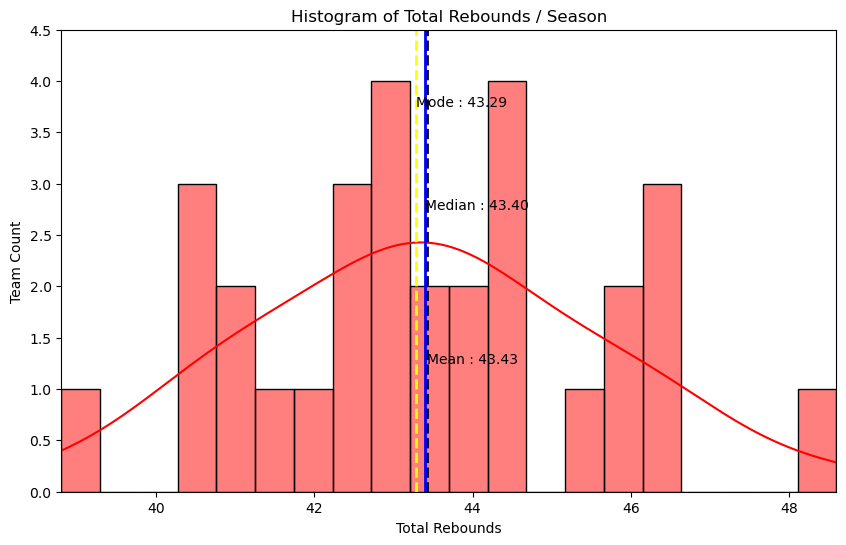
\includegraphics[scale=0.41]{TRB_image.png}
    \caption{Total Rebounds Per Game}
    \label{fig:enter-label}
\end{figure}
\vspace{\baselineskip}
\vspace{\baselineskip}

\vspace{\baselineskip}
\vspace{\baselineskip}
\vspace{\baselineskip}

\subsection{Analysis for Answering Reseach Questions}


Since we have enough data to use, let’s try to examine which
of these data are related to each other. Than we will use related
data and try to predict the winner of matches.
\vspace{\baselineskip}
\vspace{\baselineskip}
\vspace{\baselineskip}
\vspace{\baselineskip}


\subsubsection{Overview to variables}

The key to predicting the winner often hinges on the scoring frequency, primarily reflected in the total points scored by a team. Understanding the factors influencing the team's scoring ability becomes pivotal in foreseeing match outcomes. Before delving into the specifics affecting scoring, it's essential to explore the correlations between various basketball-related variables, as depicted in figure 12.
\begin{figure}[h]
    \centering
    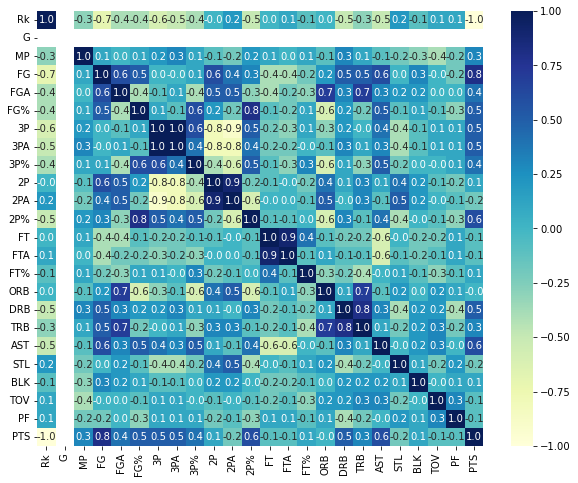
\includegraphics[scale=0.41]{heatmap.png}
    \caption{Correlation Matrix Heatmap}
    \label{fig:enter-label}
\end{figure}
\subsubsection{Overview to variables}

We'll analyze key pairs of basketball statistics to uncover potential relationships that influence game outcomes using specific features:
\vspace{\baselineskip}

\paragraph {Field Goal Percentage (FG\%) and Points Scored per Game (PTS)
}
There might be a positive correlation between FG\% and PTS. Higher FG\% often implies more effective scoring, influencing overall points per game. We anticipate a strong positive correlation, suggesting that a higher FG\% contributes to more point. We can clearly see
that there is a positive correlation between shots and goals in
Figure 13. Our correlation coefficient is 0.48.
\vspace{\baselineskip}\vspace{\baselineskip}
\begin{figure}[h]
    \centering
    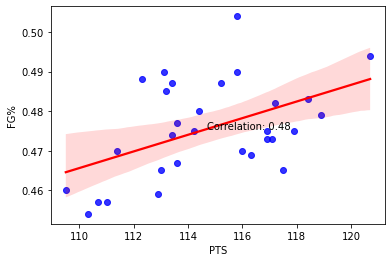
\includegraphics[scale=0.6]{pts-fg-cor.png}
    \caption{PTS and FG\% Correlation}
    \label{fig:enter-label}
\end{figure}
\vspace{\baselineskip}

\paragraph {Three-Point Percentage (3P\%) and Points Scored per Game (PTS)
}
Exploring the relationship between 3P\% and PTS. Teams with a higher 3P\% might exhibit better scoring, impacting their overall points per game. A strong positive correlation here could signify that higher 3P\% correlates with increased points. Our correlation coefficient is 0.44.
\vspace{\baselineskip}

\begin{figure}[h]
    \centering
    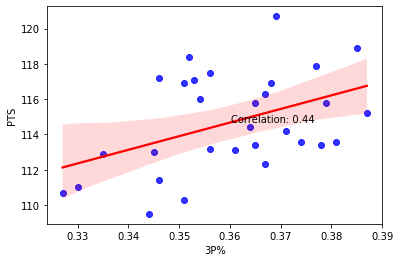
\includegraphics[scale=0.6]{3P-PTS-COR.png}
    \caption{3P\% and PTS Correlation}
    \label{fig:enter-label}
\end{figure}
\vspace{\baselineskip}\vspace{\baselineskip}
\paragraph {Free Throw Percentage (FT\%) and Points Scored per Game (PTS)}
Investigating the connection between FT\% and PTS. A correlation coefficient of 0.07 between Free Throw Percentage (FT\%) and Points Scored per Game (PTS) indicates a very weak positive linear relationship between these two variables.

\begin{figure}[h]
    \centering
    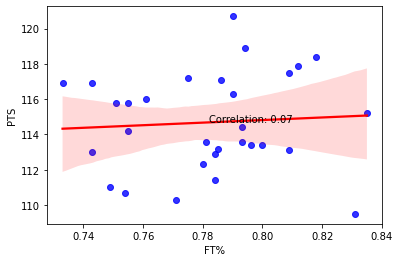
\includegraphics[scale=0.6]{FT-PTS-COR.png}
    \caption{FT\% and PTS Correlation}
    \label{fig:enter-label}
\end{figure}
\vspace{\baselineskip}
\vspace{\baselineskip}
\vspace{\baselineskip}
\vspace{\baselineskip}

\paragraph {Two-Point Percentage (2P\%) vs. Three-Point Percentage (3P\%)}
Examining the contrast between 2P\% and 3P\%. Certain teams might rely more on either 2-point or 3-point shots. A comparison would help determine if some teams heavily favor one type of scoring over the other. In the same direction can we say that 2P\% and 3P\% have a relation between them bearing in mind that both of them depends on shooting abilities. So when we look closer it seems that there is a correlation of 0.53. It denotes a moderate positive linear relationship between these features.

\begin{figure}[h]
    \centering
    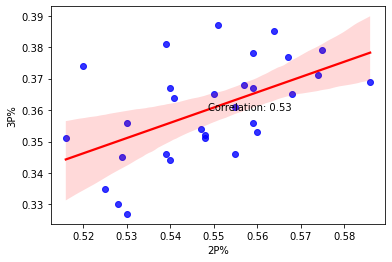
\includegraphics[scale=0.6]{2P-3P-COR.png}
    \caption{2P\% and 3P\% Correlation}
    \label{fig:enter-label}
\end{figure}

\paragraph {Assist (AST) and Turnover (TOV)}
The relationship between assists and turnovers in basketball reveals a correlation of 0.3. This correlation, while indicative of a discernible connection, implies a moderate association between these statistics. It suggests that while team play, reflected in assists, might contribute to scoring opportunities, there's also a slight propensity for higher assist rates to be accompanied by a relatively increased number of turnovers. However, the moderate correlation underlines the nuanced balance teams seek between fostering offensive teamwork and maintaining ball security.

\begin{figure}[h]
    \centering
    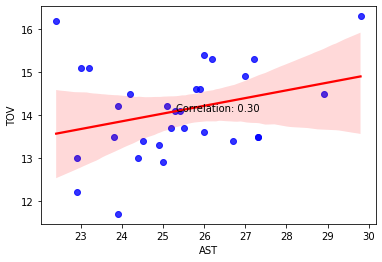
\includegraphics[scale=0.6]{AST-TOV-COR.png}
    \caption{AST and TOV correlation}
    \label{fig:enter-label}
\end{figure}


\paragraph {Steal(STL) and Block(BLK)}
Teams with better defensive statistics might concede fewer points. A negative correlation could indicate that higher defensive stats lead to fewer points allowed per game. That is the reason we will look at steal and block correlation for understanding the defensive maintenance. When we look at our graphic it says that we have a correlation of 0.1 which is low. So defensive power doesn't rely on steal and block equally.

\begin{figure}[h]
    \centering
    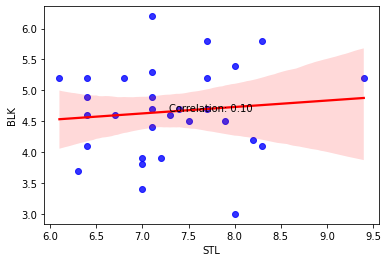
\includegraphics[scale=0.6]{STL-BLK-COR.png}
    \caption{STL and BLK correlation}
    \label{fig:enter-label}
\end{figure}
\vspace{\baselineskip}

\paragraph {Total Rebounds (TRB) and Field Goal Percentage(FG\%)}
The correlation of -0.2 between rebounds and field goal percentage (FG\%) in basketball showcases a subtle yet existing association. This negative correlation indicates that while there's a connection, it's somewhat inverse. We must bear in mind that when you miss a shot another teammate can take the offensive rebound and regain the ball. This data can show us there is a little connection between them based on offensive rebounds after the missed shot.
\vspace{\baselineskip}

\begin{figure}[h]
    \centering
    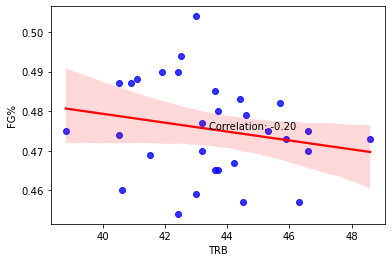
\includegraphics[scale=0.6]{TRB-FG-COR.png}
    \caption{TRB and FG\% correlation}
    \label{fig:enter-label}
\end{figure}
\vspace{\baselineskip}
\vspace{\baselineskip}
\vspace{\baselineskip}
\vspace{\baselineskip}


\subsubsection{Overview to variables}
We selected some pairs from our data and examined the
relationship between them. We will use interrelated data to
complete our analysis. We will try to determine the outcome
of the possible match of the teams using each of its associated
data. At figure 20, there is a complete pair plot of our data to
see clearly the relations between data frames.

\begin{figure}[h]
    \centering
    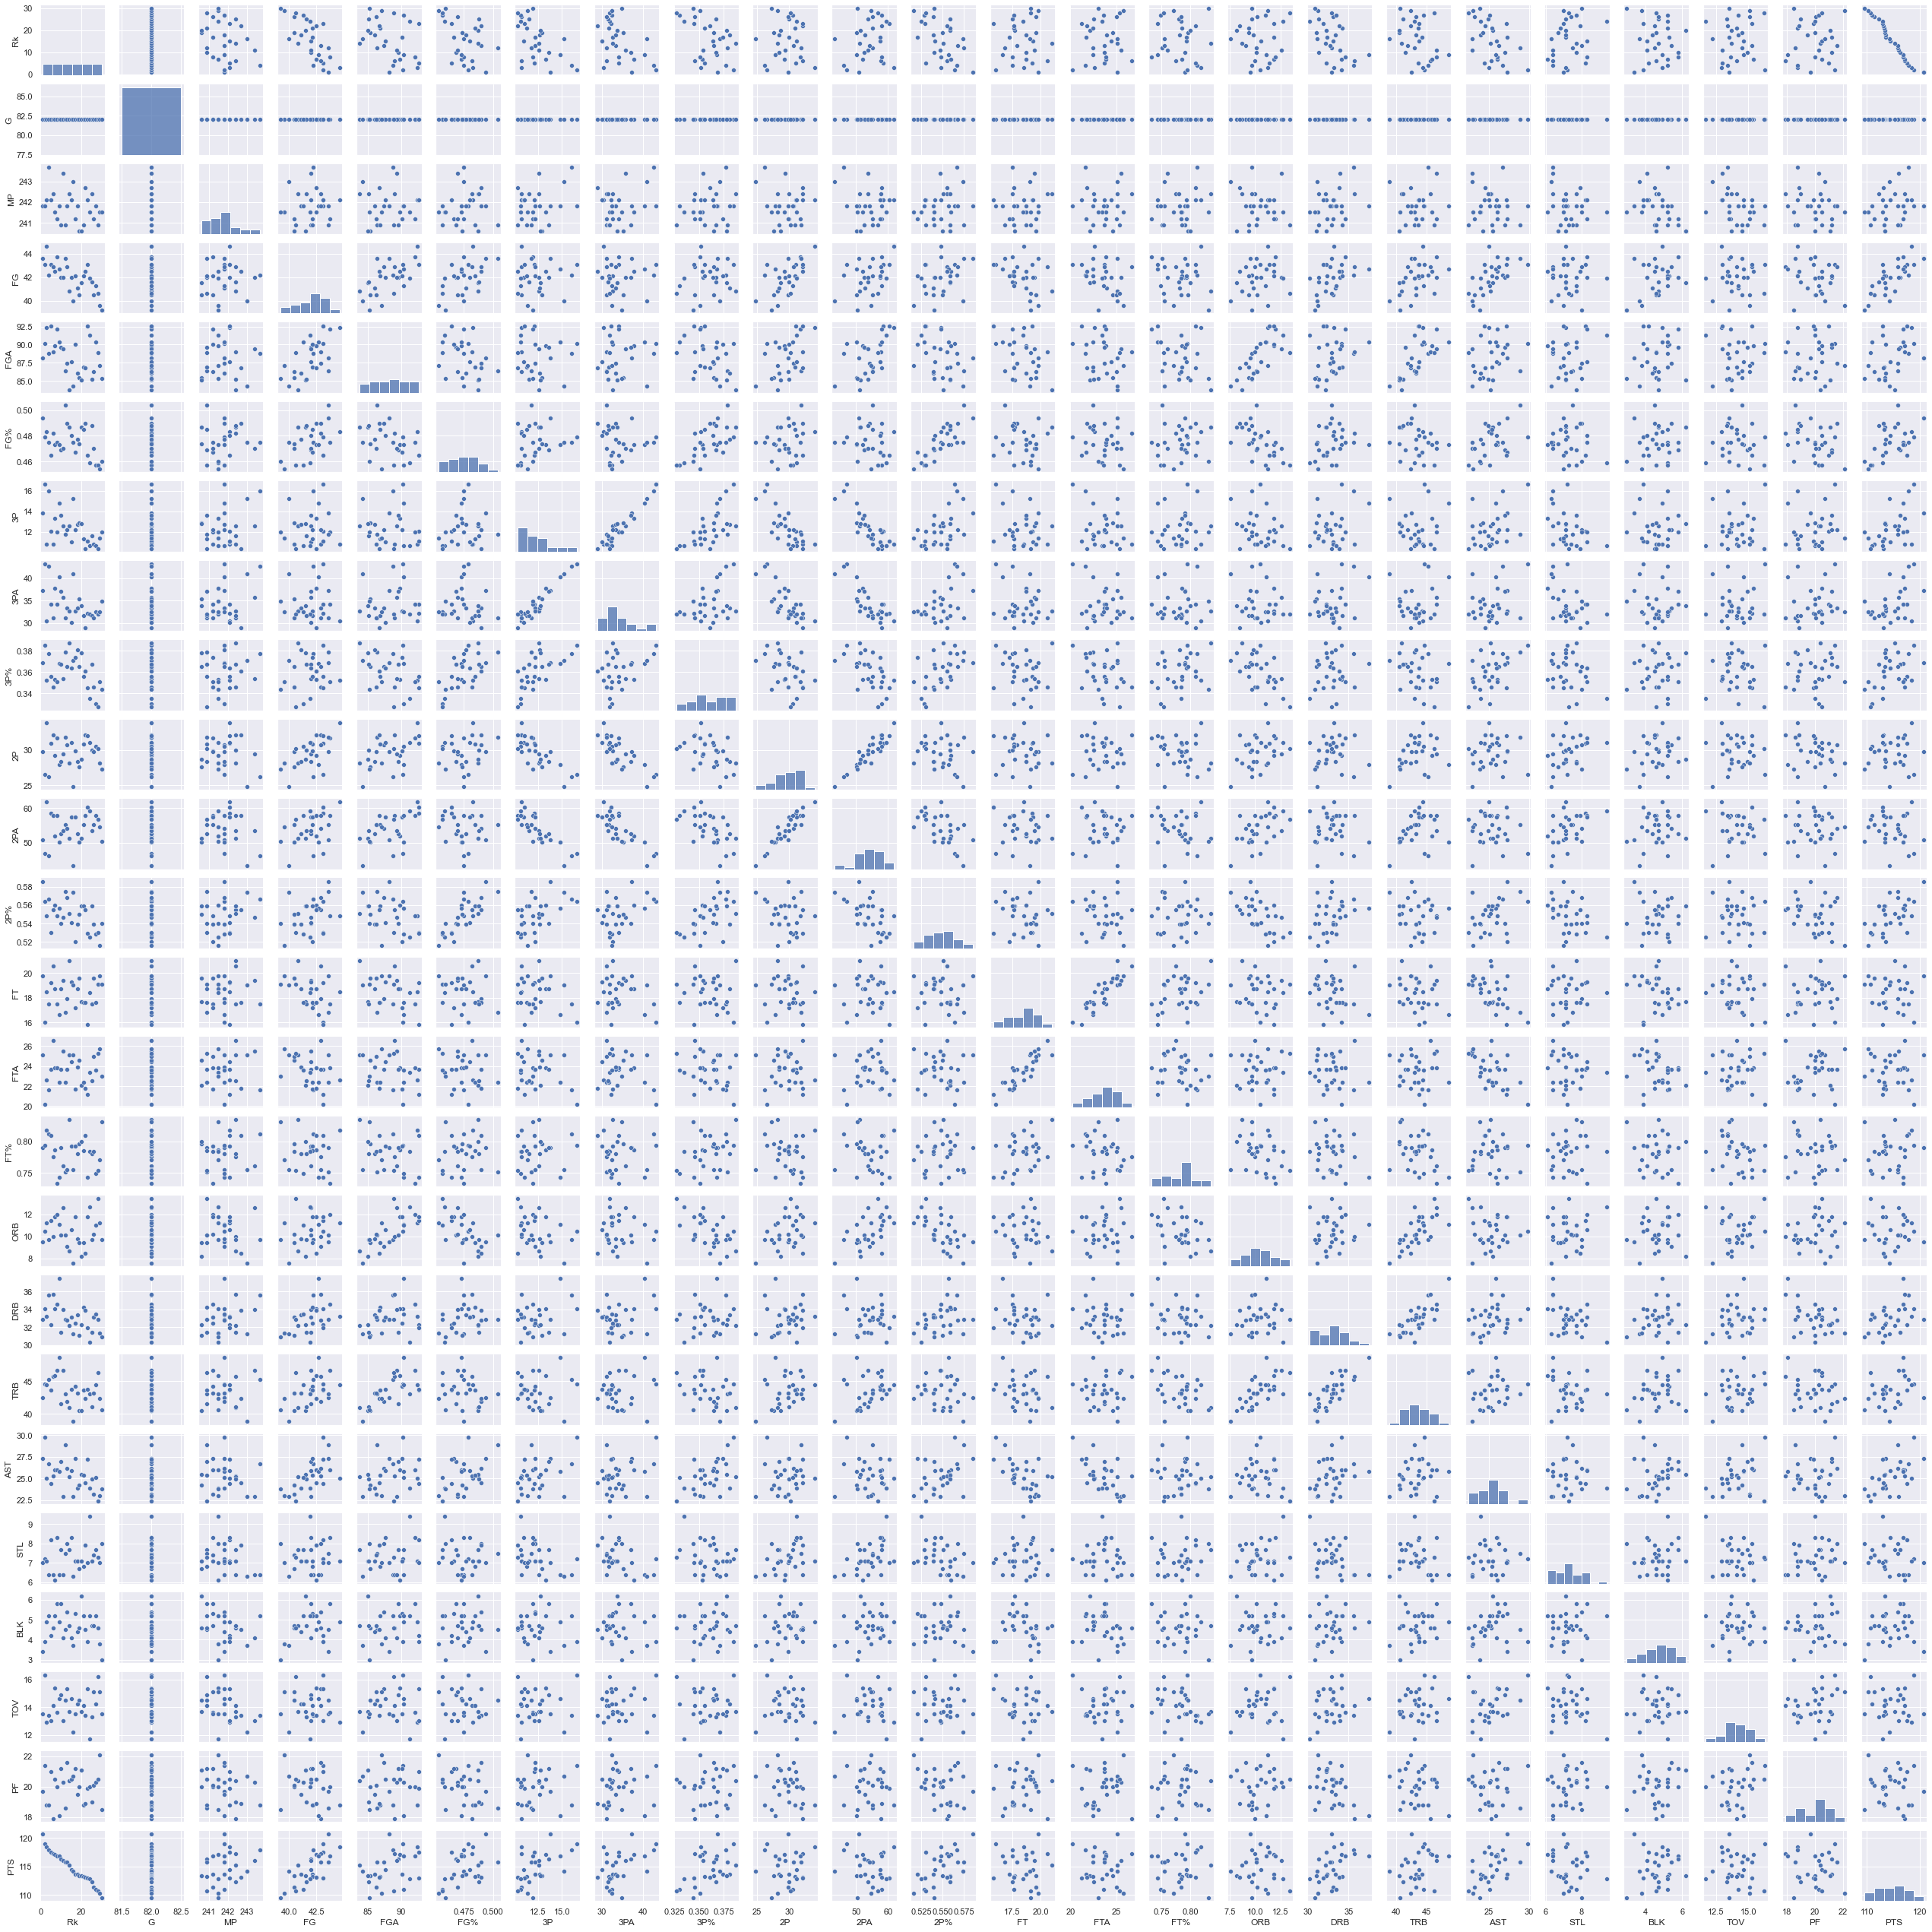
\includegraphics[scale=0.1]{tum.png}
    \caption{All Data Pairs}
    \label{fig:enter-label}
\end{figure}

\subsection{Creating and Determining A Team Score By Linear Regression}

To arrive at solid conclusions in basketball, singling out the key variable is critical. In our basketball analysis, we will use kind of a simple linear regression and identify 'Points Scored per Game' as our fundamental metric. Following this, we scrutinize attributes directly or indirectly linked to point scoring. By standardizing these variables against team averages and applying specific weightings, we establish a unique 'Team Score.' 
\vspace{\baselineskip}
\subsubsection{Determining Coefficient According To Their Effect}

Our linked values for point scoring include ’AST,’ ’FG\%,’ ’2P\%’,’3P\%’ (directly), and ’STL’,’BLK’,’TRB’ (indirectly). Allocating coefficients based on their influence, we assign ’PTS’ with a coefficient of 2, ’FG\%’ with 10, ’AST’ with 1, ’2P\%’ and 3P\% with 3, and ’BLK’, ’STL’, ’TRB’ with 0.5.\
\vspace{\baselineskip}
\subsubsection{Calculating The Team Score}
\paragraph {Formula}
\vspace{\baselineskip}
Team Score = (2 * PTS) + ( 10* FG\%) + (1* AST) + (3 * (2P\% + 3P\%)) + (0.5 * (BLK + STL + TRB))
\vspace{\baselineskip}

\paragraph {Utah Jazz}
(PTS=117.1, FG\%=0.473, AST=26, 2P\%=0.56, 3P\%=0.353, BLK=5.2, STL=6.1, TRB=45.9)
\vspace{\baselineskip}

\paragraph {Sacramento Kings}
(PTS=120.7, FG\%=0.494, AST=27.3, 2P\%=0.586, 3P\%=0.369, BLK=3.4, STL=7, TRB=42.5)
\vspace{\baselineskip}

\paragraph {Oklahoma City Thunder}
(PTS=117.5, FG\%=0.465, AST=24.4, 2P\%=0.53, 3P\%=0.356, BLK=4.2, STL=8.2, TRB=43.6)
\vspace{\baselineskip}


\paragraph {Team Scores}
Utah Jazz = 295.813, Sacramento Kings= 302.897, Oklahoma City Thunder= 294.636. When we look at the games played in 2022-2023 season between Kings and Thunder it seems that Kings won all the 3 games against Thunder, also Kings has a 3-1 result against Jazz. So according to these games they played each other it can be said that our formula has worked in general.
\vspace{\baselineskip}\vspace{\baselineskip}
\vspace{\baselineskip}


\section{Conclusion}
\vspace{\baselineskip}
\vspace{\baselineskip}

Although we've made lots of accurate predictions, it's crucial to acknowledge the inherent unpredictability in basketball. A game's outcome can hinge on numerous dynamic factors. Even with an exhaustive analysis considering various metrics, the element of chance and the spur-of-the-moment performances of players can render our analysis inconclusive. Despite recognizing the impossibility of arriving at a definite conclusion, our calculations based on diverse parameters can enhance our understanding of the team's likelihood of winning a basketball game.





\end{document}